\documentclass[a4paper,10pt,review]{elsarticle}

\usepackage{lineno,hyperref}
\modulolinenumbers[5]

% START: Inserted by AJS
\frenchspacing
\usepackage{ifxetex}
\ifxetex
  \usepackage{fontspec}
  \defaultfontfeatures{Ligatures=TeX} % To support LaTeX quoting style
  \setromanfont{Hoefler Text}
  % \setmainfont[Ligatures=TeX]{Palatino}
\else
  \usepackage[T1]{fontenc}
  \usepackage[utf8]{inputenc}
  \usepackage{lmodern}
  \usepackage{textcomp} % directly use the degree (and some other) symbol
\fi

\usepackage{fixltx2e}
\usepackage[]{graphicx}
\usepackage{ragged2e}  % for '\RaggedRight' macro (allows hyphenation)
\usepackage[pdftex]{color}
\usepackage[margin=2.75cm]{geometry}
\usepackage{upquote}
\usepackage{textgreek}
\usepackage{microtype} % place after fonts; even better typesetting for improved readability
\usepackage{xfrac} % nice fractions
\usepackage{booktabs} % nice tables without vertical lines
\setlength\heavyrulewidth{0.1em}
\setlength\lightrulewidth{0.0625em}
\usepackage[color=yellow, textsize=tiny]{todonotes}
\usepackage[font={small}, labelfont=bf]{caption} % tweaking the captions
\usepackage{gensymb}
\usepackage{amsmath,amssymb}
\usepackage{cleveref} % clever cross referencing figures and tables; last package to include
% END: Inserted by AJS
\usepackage{natbib}

\journal{Progress in Oceanography}

%%%%%%%%%%%%%%%%%%%%%%%
%% Elsevier bibliography styles
%%%%%%%%%%%%%%%%%%%%%%%
%% To change the style, put a % in front of the second line of the current style and
%% remove the % from the second line of the style you would like to use.
%%%%%%%%%%%%%%%%%%%%%%%

%% Numbered
%\bibliographystyle{model1-num-names}

%% Numbered without titles
% \bibliographystyle{model1a-num-names}

%% Harvard
% \bibliographystyle{model2-names.bst}\biboptions{authoryear}

%% Vancouver numbered
%\usepackage{numcompress}\bibliographystyle{model3-num-names}

%% Vancouver name/year
%\usepackage{numcompress}\bibliographystyle{model4-names}\biboptions{authoryear}

%% APA style
% \bibliographystyle{model5-names}\biboptions{authoryear}

%% AMA style
%\usepackage{numcompress}\bibliographystyle{model6-num-names}

%% `Elsevier LaTeX' style
% \bibliographystyle{elsarticle-num}
\bibliographystyle{elsarticle-harv}
% \bibliographystyle{elsarticle-num-names}
%%%%%%%%%%%%%%%%%%%%%%%

\begin{document}

\begin{frontmatter}

\title{Co-occurrence of marine heat waves and cold spells in nearshore and offshore regions along South Africa}

%% or include affiliations in footnotes:
\author[firstaddress]{Robert W. Schlegel\corref{mycorrespondingauthor}}
\cortext[mycorrespondingauthor]{Corresponding author}
\ead{3503570@myuwc.ac.za}

\author[secondaddress,thirdaddress]{Eric C. J. Oliver}
\author[fourthaddress]{Thomas W. Wernberg}
\author[firstaddress]{Albertus J. Smit}

% \author[mysecondaryaddress]{Global Customer Service\corref{mycorrespondingauthor}}

\address[firstaddress]{Department of Biodiversity and Conservation Biology, University of the Western Cape, Private Bag X17, Bellville 7535, South Africa}

\address[secondaddress]{ARC Centre of Excellence for Climate System Science, The University of New South Wales, Sydney, Australia}

\address[thirdaddress]{Institute for Marine and Antarctic Studies, University of Tasmania, Hobart, Australia}

\address[fourthaddress]{UWA Oceans Institute and School of Plant Biology, The University of Western Australia, Crawley, 6009 Western Australia, Australia}

\begin{abstract}
The term marine heat wave (MHW) was first coined in 2013 with no central definition having been agreed upon before. This lack of a definition had led to an inability of different research groups to compare their findings on this phenomenon before 2013. In order to assuage this issue, a research team has recently created a definition for MHWs that will be valid anywhere in the world. We have taken this algorithm and applied it to the \emph{in situ} time series available for the coast of South Africa that are longer than 10 years and with at least 90\% complete daily records. It was also decided to apply the algorithm to cool temperatures and investigate the presence of marine cold spells (MCSs). We found that MHWs and MCSs can be found along the entire stretch of South Africa's coastline and with some temporal and spatial agreement between the largest events detected. MHWs occur more often, last longer than MCSs and have greater cumulative intensities. There was little variance in the cumulative intensity [\degree C \texttimes~days] around the mean for MHWs and MCSs however, several were much larger and there tended to be specific time series that displayed more dramatic results than others. The coastline was further divided into three sections (west, south, and east) to investigate the effect of geography on MHWs and MCSs and it was found that the south coast experiences more, longer and more intense MHWs and MCSs than the other two coastlines. The mechanism driving the higher intensity of events on the south coast, which is much greater than the other coasts, requires further study. The largest three MHWs of most time series along the coast of South Africa have occurred in the second half of the time series whereas the largest three MCSs have occurred in the first half. These same calculations were conducted for offshore temperatures from NOAA optimally interpolated sea surface temperature (OISST) data, too. It was found that the proportion of co-occurrence between \emph{in situ} and OISST data ranged from 0.5--0.0 for each coastline with co-occurrence rates being the largest on the south coast. Few time series showed co-occurrence amongst the 50\% largest events.
\end{abstract}

\begin{keyword}
marine heat waves \sep marine cold spells \sep OISST \sep \emph{in situ} data \sep co-occurrence \sep climate change \sep extreme events \sep South Africa \sep coastal
\end{keyword}

\end{frontmatter}

\linenumbers

\section{Introduction}

Over the past three decades, global-scale anthropogenically mediated warming has negatively affected marine and terrestrial realms with far reaching consequences for humanity and natural ecological functioning. Although climate change is generally understood as a gradual long-term rise in global mean surface temperature \citep{IPCC2014}, which will continue for decades or centuries, it is generally the associated increase in frequency and severity of extreme events that affects humans and ecosystems alike in the short-term \citep{Easterling2000}. Impacts are often sudden with catastrophic consequences. Such extreme events include droughts, floods, wind storms, tropical cyclones, heat waves and cold spells. `Pulse' events exceeding certain thresholds of frequency, intensity (extremeness), duration, timing and rate of onset (abruptness) can drive punctuated perturbations to species distributions, which eventually modify the structure and function of ecosystems \citep{Wernberg2013, Rehage2016}, and the recognition to focus more on events and less on trends has emerged as a recent direction of climate change research \citep{Jentsch2007}. The focus of this paper is on marine thermal events that are extreme with respect to the seasonal climatology. They may be anomalously warm (marine heat waves, MHW; \emph{sensu} Hobday et al. 2016), or anomalously cold (marine cold spells, MCS; introduced here). While MHWs are becoming reasonably well known by virtue of their increasing frequency and intensity, there is less information about the ecological effects of extreme cold events. There is also a paucity of information about their drivers. [\textbf{What we need to do to address Eric's first concern about ``Given that we can’t really say much about the long-term trends given that most stations are in the 10-20 years range of data record length'' is make the case that these events are increasing offshore, but that this offshore increase is not necessarily related to an increase inshore due to the decoupling of the meso-scale from the local scale extreme events. Although not all of our inshore series are long enough, some of them are (Port Nolloth, Sea Point, Muizenberg, Gordon's Bay) and here we can provide data to show that they are/are not increasing. Perhaps I should also do a proper analysis of the OISST time series to indicate that the temperatures are indeed increasing with time.}]

[\textbf{W.r.t. Eric's comment about ``extreme events happen regardless of climate change. This paper mostly focusses on the mean state not the changes''... I think Rob has now looked at the increasing frequency of the extreme events in the OISST data, and I think we should do the same with the \emph{in situ} time series I mentioned in my comment above. W.r.t. the extrme events: the prediction is that in a changing climate the extreme warm (cold) events will become more common (less common), while under a static long-term trend their frequecy will be homogeneous w.r.t. time. This is a necessary outcome of the way that the extreme events are calculated.}]

The concept of heat waves is usually applied to atmospheric phenomena where vague definitions such as ``a period of abnormally and uncomfortably hot and usually humid weather'' are invoked \cite{Glickman2000}, but there are also precise definitions based on statistical properties and other metrics of the temperature record that are relative to location and time of year (e.g. \cite{Meehl2004, Alexander2006, Fischer2010, Fischer2011}). Recent years have seen investigations of heat waves in the ocean due to them becoming more frequent over time (e.g. \cite{Mackenzie2007, Selig2010, Sura2011, Lima2012, DeCastro2014}). Well documented marine heat waves (MHW) have occurred in the Mediterranean in 2003 (e.g. \cite{Black2004, Olita2007, Garrabou2009}), off the coast of Western Australia in 2011 (e.g. \cite{Feng2013, Pearce2013, Wernberg2013}), in the north west Atlantic Ocean in 2012 (e.g. \cite{Mills2012, Chen2014, Chen2015} and now the ``Blob'' from 2014 to 2016 in the north east Pacific Ocean \cite{Bond2015}. The extreme temperatures from these events, and others like them, may have wide ranging negative impacts upon the local ecology for the regions in which they occur. For example, the 2003 Mediterranean heat wave may have affected up to 80\% of the gorgonian fan colonies in certain areas of this sea \cite{Garrabou2009}, whereas the 2011 event off the west coast of Australia has been recognized as being a driving factor in the regime shift there from temperate kelp forests to the beginnings of a coral reef system \cite{Wernberg2013}. Because the inquiry into MHWs is a relatively new endeavour none of these studies provided adequate definitions for what constitutes a MHW, and to that end Hobday et al. (2016) \cite{Hobday2016} have defined it as ``a prolonged discrete anomalously warm water event that can be described by its duration, intensity, rate of evolution, and spatial extent''. By applying the MHW definition to the aforementioned events, Hobday et al. (2016) \cite{Hobday2016} were able to derive statistical features of the MHWs, such as their frequency along a time series and maximum and cumulative intensity. Whereas extreme hot events may be demonstrably damaging to organisms and ecosystems, extreme cold events also have the potential to negatively impact organisms and ecosystems.

MCSs are analogous to MHWs, but they are of opposite sign. MCSs are projected to become less frequent under future climatic scenarios, but there are also examples of them becoming more frequent in some localities \cite{Gershunov2008, Matthes2015}. They are frequently lethal \cite{Woodward1987} and are known to have caused mass fish \cite{Gunter1941, Gunter1951, Holt1983} and invertebrate \cite{Gunter1951, Crisp1964} kills, the death of juvenile and sub-adult manatees \cite{OShea1985, Marsh1986} as well as affecting organismal physiological tolerances, life history strategies, and habitat requirements \cite{Ellis2015}. Cold temperatures are therefore very important in setting species distribution limits, particularly limiting their range north- or southwards towards high latitudes \cite{Firth2011}, and the timing of the onset of the growing season \cite{Jentsch2007}. At an ecosystem level there is still a paucity of information on effects of MCSs, but it is easy to postulate how population-level consequences might aggregate to drive whole ecosystem responses (e.g. \cite{Kreyling2008, Rehage2016}). Indeed, the range contractions of ecosystem engineer species such as mussels have been shown to relate to MCSs (e.g. \cite{Firth2011, Firth2015}).

Some of the MCSs known to have had impacts on populations and ecosystems were caused by atmospheric cold spells that affect the intertidal biota (e.g. \cite{Gunter1941, Firth2011}) and not by seawater. Here we focus on MCSs measured in seawater. This may imply local events (i.e. extreme atmospheric cold spells that perturb the seawater locally) or broad-scale drivers. The driver of the MCSs localised to the coast, as we have already suggested, is hypothesised to be coastal weather phenomena. But what mechanism might explain coastal MCSs originating from offshore or by oceanic processes? Large-scale atmospheric-oceanographic coupling is very likely being affected by global warming, which is projected to cause the intensification of upwelling favourable winds and consequently the intensification and increasing frequency of upwelling (see Garciá-Reyes et al. 2015 for a review of this and alternative hypotheses). The question then is, could an intensification of upwelling be attributed to coastal MCSs, or are they linked to local coastal atmospheric forcing? Little research yet exists that investigates this question other than to link anoxia and other negative factors from problematic phytoplankton blooms caused by extreme upwelling events to create lethal conditions for species living within upwelling regions (e.g. \cite{Laboy-nieves2001}). Whereas anoxia is a problem attributable to phytoplankton blooms themselves \cite{Diaz2008} and not the extreme cold temperatures \textit{per se}, if a relationship can be shown between MCSs and anoxia resulting from algal blooms it would provide extremely valuable insight into how coastal ecosystems respond to climatic change. Furthermore, since mass mortalities and ecosystem change may result directly from MCSs, a mechanistic understanding of their drivers will be invaluable. To this end it serves as a constructive first step to study the prevalence of MCSs with respect to different kinds of oceanic forcing mechanisms.

Hobday et al. (2016) \cite{Hobday2016} applied their MHW framework to \sfrac{1}{4}\degree~NOAA optimally interpolated sea surface temperature (hereafter referred to as OISST; \cite{Reynolds2007}) data, but warned users to be cognisant that different data sets would provide different kinds of information pertaining to the heat waves. Our aims here are two-fold. Firstly, we apply the MHW (MCS) definition to datasets of \emph{in situ} and gridded SST temperature time series collected at different scales along the South African coast for three different coastal sections, each variously forced by the Agulhas and Benguela Currents and regional aspects of the coastal bathymetry and geomorphology. These regional drivers of the thermal regime (east, south and west coast) coupled with local modifications (coastal vs. offshore) can be expected to impart different thermal signatures on the temperature data sets and manifest in differences in the metrics of MHWs (MCSs). Secondly, we aim to discuss the significance of MHWs (MCSs) within the context of the data sets’ inherent differences and the various dynamical properties that then emerge because of the regional oceanographic context, so as to provide a mechanistic understanding of the nature and origin of MHWs (MCSs) in three oceanographically distinct ocean/coastal regions.

To add a mechanistic understanding of the drivers of MHWs (MCSs) manifesting in the coastal environment, we hypothesised that coastal MHW (MCS) events could either be coupled with synoptic scale processes perturbing the offshore region at scales of 100s of kms, or originate solely at a local scale as isolated incidents. Investigating the former possibility required the assessment of concurrent gridded SSTs derived from daily OISST data product, extracted for the bounding boxes in \Cref{fig:Figure1}, averaged spatially, and lagged or led by a number of days relative to the onset of the events at the coast. This analysis centres around the top three MHWs (MCSs) ranked with respect to cumulative intensity for each of 21 coastal sites. The rates of co-occurrence of coastal with mesoscale MHWs (MCSs) are used in part to understand how many of the extreme events detected in all three coastal sections originate at the coast or are artefacts of warming (cooling) in the respective currents. We think that this approach will yield considerable insight into the nature and variability of the thermal regime of nearshore seawater.

\begin{figure}
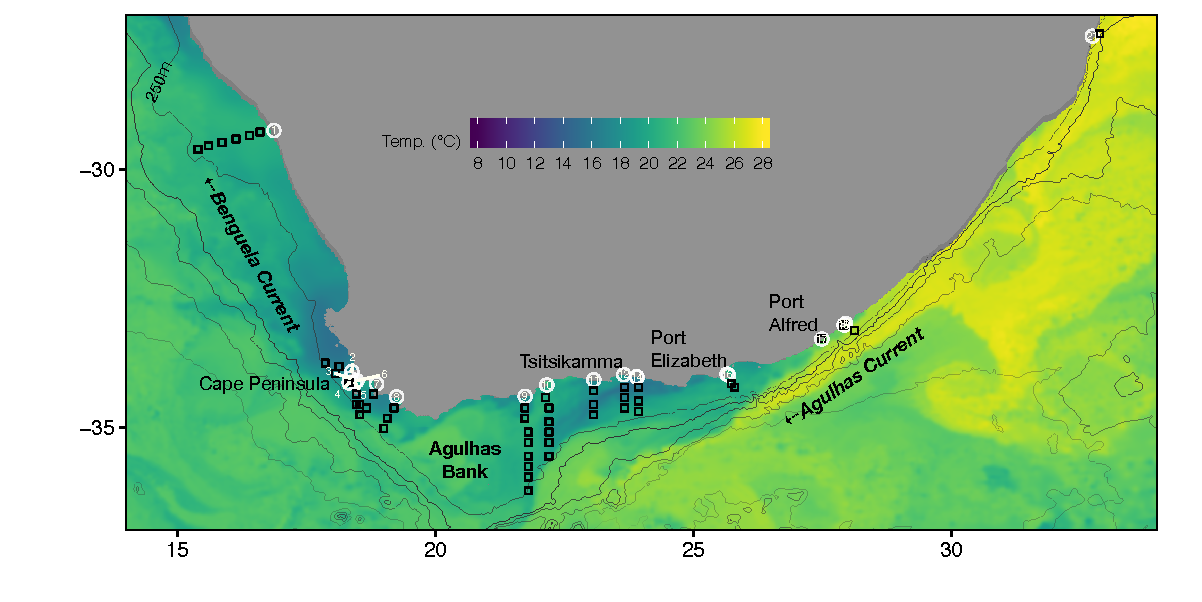
\includegraphics[width=1.0\textwidth]{figure1_1km_labeled.pdf}
\caption{Map of South Africa showing the bathymetry (only the 250 m isobath is indicated), the location of the \emph{in situ} thermal time series shown with circles and approximations of the pixels used along the shore-normal transects from the daily \sfrac{1}{4}\degree~NOAA OISST \cite{Reynolds2007} shown with black boxes. The SST field was derived from the JPL G1SST 1 km blended SST product and shows the state of the ocean on 2016-02-14. Sites 5, 6 and 7 are to the east of the Cape Peninsula and are situated along the shores of False Bay. The Agulhas Current along the east coast of the country is visualized here in a yellowish colour as a jet of relatively warmer water projecting in a south-westerly direction, and hugging the continental shelf. The blueish patches north of the Cape Peninsula represent upwelled water. Some upwelled water may also be present around Sites 14 (Tsitsikamma) and 15--16 (Port Elizabeth).} \label{fig:Figure1}
\end{figure}

\section{Methods}
\subsection{Study region}
The variety of oceanographic features around the \emph{ca}. 2,700 km long South African coastline provides a natural testing bed for the potential effects of different forcing mechanisms on the occurrence of MHWs and MCSs. Annual mean (SD) coastal seawater temperatures range from 12.3 (1.2)\degree C at the western limit near the Namibian border (Site 1) to 24.4 (2.0)\degree C in the east near the Mozambican border (Site 21), and our study sites were selected to cover this full range (\Cref{fig:Figure1}). We classify the coastline into three regions based on their major oceanographic features, their temperature characteristics, and aspects of the underlying continental shelf. The first is the west coast region dominated by the Benguela Current, which forms an Eastern Boundary Upwelling System (EBUS) \cite{Hutchings2009}. Seasonal upwelling is maintained by prevailing south-easterly trade winds. Evenly low temperatures are especially noticeable at upwelling cells over a relatively narrow continental shelf in the region northwards of the Cape Peninsula to Cape Columbine. The west coast defines a cool temperate regime, with the range of monthly mean temperatures at most sections intermediate between cold temperate and warm temperate \cite{Luning1990}. The second region is the warm temperate (\emph{sensu}  \cite{Luning1990}) east coast where the influence of the south-westerly flowing warm Agulhas Current flowing tightly along the narrow continental shelf (except for the Natal Bight) is strongly felt. This stretch of coastline is spatially homogeneous with respect to temperature and characterised by a moderate amount of seasonal variation. Although the Agulhas Current retroflects back into the southern Indian Ocean \cite{Hutchings2009} just south of the much wider and cooler Agulhas Bank \cite{Roberts2005}, its influence extends as far west as False Bay (Sites 5--21; \Cref{fig:Figure1}). The third coastal region is that overlying the Agulhas Bank. Although also warm temperate, it experiences a much larger range in annual temperature and variability compared the west and east coast regions, which is in part influenced by the retention and cooling of Agulhas Current water on the bank, the presence of some current-driven upwelling cells along this coastline (Sites 15--17) \cite{Roberts2005}, and because of the effects of embayments and capes throughout the region.

\subsection{Temperature data}
We use two sources of seawater temperature data. The first dataset is comprised of 127 records of \emph{in situ} temperature records of daily measurements for up to 40 years in duration with a mean duration of \emph{ca}. 19 years. Whereas these \emph{in situ} time series are generally shorter than the recommended 30 year minimum \cite{Hobday2016} and have some small amounts of missing data, it is our opinion that the benefit of using \emph{in situ} data over satellite data is that they give a better representation of the thermal characteristics near the coastline, a region where satellite SST measurements have been shown to perform poorly (e.g. \cite{Smale2009, Castillo2010}). In a South African context, Smit et al. (2013) \cite{Smit2013} have shown that satellite SST data display a warm bias as large as 6\degree C over \emph{in situ} temperatures in the nearshore environment. In an attempt to compromise between the proscribed requirements in Hobday et al. (2016) \cite{Hobday2016} of a 30 year minimum and no missing data, all time series under 10 years in length were eliminated. Next, our 127 time series were screened and those missing more than 10\% of their daily values were removed, leaving a total of 21 time series. Care was taken to select continuous series with as few as possible consecutive missing values, since having regions in the data with more than two consecutive missing data points interferes with the identification of the anomalous events (see below). These stations were classified into three coastal sections defined by properties of their oceanography and biogeography \cite{Smit2013}. The meta data for these time series and the coastal sections they were aggregated into may be found in Table S1 \todo{The Supplementary material must still be put together.} and the site localities are displayed spatially in \Cref{fig:Figure1}.

The second set of temperature data used in this study are the daily \sfrac{1}{4}\degree~NOAA optimally interpolated sea surface temperature (OISST; \cite{Reynolds2007}) derived from the Advanced Very High Resolution Radiometer (AVHRR). To compare the OISST and \emph{in situ} time series, shore-normal transects were drawn from each of the 21 sites extending to the 200 m isobath. The OISST data were then extracted at each of the roughly 25~\texttimes~25 km pixels along these transects, shown as black boxes in \Cref{fig:Figure1}. Where the shelf was less than 25 km wide (Sites 17--21) the nearest `ocean pixel' to the \emph{in situ} time series coordinate was used. The individual time series within each pixel were then averaged along each transect corresponding to the 21 \emph{in situ} sites. This produced 21 OISST time series that could then be analysed for MHWs (MCSs) in the same way as the \emph{in situ} data. Note that the OISST time series had valid data covering 1982--2014 which did not match exactly the coverage by individual \emph{in situ} sites.

\subsection{Defining and calculating MHWs and MCSs}
MHWs are ``discrete prolonged anomalously warm water events in a particular location.'' Here we introduce the opposite but analogous concept of a Marine Cold Spell (MCS), which is calculated in the same manner as a MHW, except that events are detected as deviations below a seasonally varying anomalously low threshold relative to the site’s climatology. Although MCS intensities are calculated as negative values (i.e. anomalies) they are reported here as absolute values.

A Python script (https://github.com/ecjoliver/marineHeatWaves; see Hobday et al. (2016) \cite{Hobday2016}) was used to calculate the MHWs and MCSs for both the \emph{in situ} and OISST time series, producing the metrics in \Cref{table1}. The individual events detected and their attendant statistics were meaned into a series of annual values. These annual values were then meaned for each coastal section for later comparison.

\begin{table}[]
\caption{\small Metrics of MHWs and their descriptions as used by Hobday et al. (2016) \cite{Hobday2016}. In the case of MCSs, values are calculated with respect to the 10th percentile and absolute intensity values are reported.}
\label{table1}
\centering
\tiny
\begin{tabular}{ll}
\hline
 Name [unit] & Definition \\
 \hline
  Count [no. events per year] & \emph{n}: number of heatwaves per year \\
  Duration [days] & \emph{D}: Consecutive period of time that temperature exceeds the threshold \\
  Maximum intensity [\degree C] & \emph{i\textsubscript{max}}: highest temperature anomaly value during the MHW \\
  Mean intensity [\degree C] & \emph{i\textsubscript{mean}}: mean temperature anomaly during the MHW \\
  Cumulative intensity [\degree C x days] & \emph{i\textsubscript{cum}}: sum of daily intensity anomalies \\
  \hline
  \end{tabular}
\end{table}

To detect the individual events, a climatological mean and 90th and 10th percentiles were calculated for each day of the year by pooling all data within an 11-day window across all years. MHWs (MCSs) were detected as periods of time when temperatures exceeded the 90th (10th) percentile for at least five days. The implication is therefore that MHWs (MCSs) could develop in winter (summer) months. Since our \emph{in situ} time series are of differing lengths we calculated the climatology over all available years; in the case of the OISST data, climatologies were calculated over a 30-year base period from 1982--2012. Furthermore, the algorithm found discrete events with well-defined start and end dates, but `breaks' between events lasting $\leq$2 days followed by subsequent $\geq$5 day events were considered as continuous events. Once events were defined, a set of metrics were calculated including maximum and mean intensity (measured as anomalies relative to the climatological mean), duration (time between start and end dates), and cumulative intensity (the integrated intensity over the duration of the event, analogous to degree-heating-days).

Because MHWs (MCSs) are thus calculated by percentiles rather than maximum values centered around a window of time with respect to the Julian day, any time of year could be shown to be experiencing a MHW (MCS). This is an important consideration as unusually warm waters occurring during the winter months of a year, the time when many species need cold water for effective spawning spore release, can have a negative effect on the recruitment success of that population for the year \cite{Wernberg2011}.

It is important to understand that MHWs can result from a combination of atmospheric forcing and oceanic processes, but that the approach here aims only to shed light on the oceanic drivers by virtue of the inclusion of mesoscale OISST data linked with the coastal \emph{in situ} data sets.

In order to better understand the potential impact mesoscale phenomena have on coastal events, the rates of co-occurrence between the MHWs (MCSs) found within each time series between the two datasets were compared. This was initially done by taking each event (warm and cold) within an \emph{in situ} time series and looking for an event occurring within the OISST time series at the same site within a certain period of time before the \emph{in situ} date. These co-occurrence proportions were then used to describe how often the mesoscale oceanography off the coast pre-empted the extreme events occurring along the coastline. All events occurring on dates not found in the matching time series were removed from this calculation. The sum of events found to occur within similar times was then divided by the total number of \emph{in situ} events checked against the OISST data to produce a co-occurrence proportion. The proportions of co-occurrence were then recalculated controlling for the amount of lag used when comparing the two different datasets for concurrent events, as well as the directionality used for this comparison. In other words, a range of lag from 2--14 was used for each site to see how far apart events generally occurred and the lag period used was also applied only after the \emph{in situ} date, as well as both before and after the date, effectively doubling the range of the lag. This allowed us to see how often the \emph{in situ} event pre-empted the mesoscale event as well as seeing broadly the amounts of co-occurrence occurring between the two data sets.

Besides controlling for the length and direction of lag, the size of the events themselves (ranked by cumulative intensity) were compared. This was accomplished by controlling the pool of events with which to compare the datasets per site in steps of 10th percentiles. This progressively removed smaller events until only the larger events were being compared. This allowed us to track the co-occurrence of only the largest events, reducing the overall proportion of co-occurrence found within each site as caused by the large amount of smaller events occurring at similar times as other larger events.

The top three MHWs (MCSs) for each \emph{in situ} and OISST time series as defined by cumulative intensity were also noted in order to visually compare the co-occurrence of events in detail, both within and between the different datasets.

Given that the anthropogenic forcing of climate change is predicted to increase the temperature of most of the ocean over time, it stands to reason that, as a function of the 90th and 10th percentiles, one would expect to see the larger MHWs near the end of the time series, and the larger MCSs near the beginning. \todo{Was this in fact done? I have started writing the code to quantify this, but need to finish it off.} This can be tracked visually by looking at the top three warm and cold events for each time series.

\section{Results}

\subsection{Events}
One can see in \Cref{table2} that the \emph{in situ} time series show that the typically cooler west coast experiences the most MHWs per year, and that these are longer and more intense on average than those along the other two coastal sections. Whereas the east coast experiences slightly more MCSs per year than the other two coastal sections, it is the volatile south coast that experiences the longest and most intense MCSs. There is no significant difference between the annual count of events for each coastal section (df = 2, F = 0.727, \emph{p} = 0.48) or between the count of MHWs and MCSs (df = 1, F = 0.732, \emph{p} = 0.39). There is a significant difference between the coastal sections for the duration of events (df = 2, F = 8.907, \emph{p} < 0.01) but no significant difference between the event types themselves (df = 1, F = 0.722, \emph{p} = 0.39). The intensity of events is significantly different between each coastal section (df = 2, F = 57.55, \emph{p} < 0.01) and the type of events (df = 1, F = 5372, \emph{p} < 0.01).

\begin{table}[]
\caption{\small The mean(sd) annual values for event frequency, duration and intensity for MHWs and MCSs for each coastal section as calculated from the \emph{in situ} time series. All individual events were first aggregated into annual means before being averaged into overall mean values for each coastal section.}
\label{table2}
\centering
\tiny
\begin{tabular}{lcccccc}
\hline
 coast & MHW [count] & duration [days] & intensity [\degree C] & MCS [count] & duration [days] & intensity [\degree C] \\
 \hline
  all & 1.6(1.8) & 9.3(5.1) & 2.65(0.79) & 1.5(1.7) & 9.0(5.1) & 2.79(1.09) \\ 
  west & 1.8(1.9) & 9.1(3.9) & 2.86(0.90) & 1.5(1.9) & 8.5(5.2) & 2.32(0.58) \\ 
  south & 1.5(1.8) & 9.8(6.1) & 2.50(0.65) & 1.5(1.6) & 9.7(5.5) & 3.08(1.22) \\ 
  east & 1.5(1.7) & 7.7(2.2) & 2.85(0.89) & 1.6(1.6) & 7.1(1.9) & 2.37(0.67) \\ 
  \hline
  \end{tabular}
\end{table}

Results from the analysis of the OISST data (\Cref{table3}) show that there is a significant difference from the \emph{in situ} data for count (df = 1, F = 50.272, \emph{p} < 0.01) and duration (df = 1, F = 17.575, \emph{p} < 0.01) of events but not mean intensity (df = 1, F = 0.117, \emph{p} = 0.73). The mean annual count and duration of MHWs and MCSs are greater than their \emph{in situ} counterparts for all coastal sections whereas the intensity of both event types on all coastal sections are less than the results of the \emph{in situ} data. With this in mind we still see that the pattern of MHW and MCS event sizes along the coastline differs from the \emph{in situ} data, too. The largest annual number of MHWs in the OISST data occur on the warmer east coast whereas the longest MHWs are occurring on the volatile south coast with the most intense events nearly split between the west and south coasts respectively. The cooler west coast sees the most frequent occurrence of MCSs with the OISST data. The longest MCSs are occurring on the south coast, same as the \emph{in situ} data; however the most intense MCSs are seen off the east coast. There is no significant difference between the annual count of events per coast (df = 2, F = 0.542, \emph{p} = 0.58) or event type (df = 1, F = 0.155, \emph{p} = 0.69). The duration of the events in the different coastal sections differe significantly from one another (df = 2, F = 9.534, \emph{p} < 0.01) whereas the duration of the event types does not (df = 1, F = 0.055, \emph{p} = 0.81). Lastly, as with the \emph{in situ} data, the intensity of events differs significantly between each coastal section (df = 2, F = 16.17, \emph{p} < 0.01) and the type of event (df = 1, F = 17645, \emph{p} < 0.01).

\begin{table}[]
\caption{\small The mean(sd) annual values for event frequency, duration and intensity for MHWs and MCSs for each coastal section as calculated from the OISST time series. All individual events were first aggregated into annual means before being averaged into overall mean values for each coastal section.}
\label{table3}
\centering
\tiny
\begin{tabular}{lcccccc}
\hline
 coast & MHW [count] & duration [days] & intensity [\degree C] & MCS [count] & duration [days] & intensity [\degree C] \\
 \hline
  all & 2.2(2.1) & 10.2(5.4) & 1.72(0.33) & 2.2(2.6) & 10.2(5.1) & 1.83(0.52) \\ 
  west & 2.1(1.8) & 10.9(6.7) & 1.75(0.41) & 2.3(2.7) & 9.8(6.6) & 1.87(0.61) \\ 
  south & 2.2(2.1) & 10.6(5.5) & 1.74(0.29) & 2.1(2.7) & 10.7(5.0) & 1.79(0.45) \\ 
  east & 2.5(2.3) & 8.3(2.4) & 1.64(0.33) & 2.2(2.2) & 9.4(3.4) & 1.93(0.61) \\ 
  \hline
  \end{tabular}
\end{table}

\subsection{Top three events}\todo{Still need to add significant differences}
The mean annual statistics shown in \Cref{table2} and \Cref{table3} give a broad view of the events occurring along the coastline; however, examining the largest MHWs and MCSs aids in our understanding of which coastlines may have the most extreme events. The ranking of these events is based on the cumulative intensity statistic as explained in \Cref{table1}. The three largest MHWs that occurred within the \emph{in situ} dataset were all on the south coast (\Cref{table4}), showing that 1999 was a particularly hot year. The size of the south coast events are larger than those occurring along the west coast, with the largest three MHWs on the east coast being much smaller than those occurring on the south coast (\Cref{table4}). The cumulative intensity of the entire coastline and each section individually may be calculated for both datasets from \Cref{table2} and \Cref{table3} by multiplying the duration by the intensity. When calculating the mean cumulative intensity of MHWs from the \emph{in situ} data for the entire coastline by the individual events and not the annual means we see that mean is 26.11(\degree C x days) with a standard deviation of 24.37(\degree C x days), meaning that the largest MHWs seen on the south and west coasts are significantly larger than the coastal average.

\begin{table}[]
\caption{\small The three largest MHWs per coast from the \emph{in situ} data. The coast column shows in which coastal section the event occurred. The site column gives the name of the site, as seen in \Cref{fig:Figure2}, which gives the index number necessary to find it's location along the coastline in \Cref{fig:Figure1}. The start date column gives the day on which the event began and the duration (days) column shows how many days the event lasted for. The intMean column shows the mean intensity of the event and the intCum column shows the cummulative intensity, as caluclated in \Cref{table1}.}
\label{table4}
\centering
\tiny
\begin{tabular}{llcccc}
\hline
 coast & site & start date & duration [days] & intMean [\degree C] & intCum [\degree C x days] \\ 
  \hline
  west & Sea Point & 1996-01-04 & 40 & 3.08 & 123.20 \\ 
  west & Sea Point & 2005-05-21 & 39 & 2.56 & 99.66 \\ 
  west & Sea Point & 1975-12-30 & 38 & 2.62 & 99.41 \\ 
  south & Muizenberg & 1999-12-01 & 98 & 3.17 & 310.30 \\ 
  south & Mossel Bay & 1993-06-25 & 97 & 1.77 & 171.30 \\ 
  south & Muizenberg & 1999-10-20 & 35 & 4.47 & 156.40 \\ 
  east & Nahoon Beach & 1995-10-14 & 18 & 5.18 & 93.31 \\ 
  east & Eastern Beach & 1985-12-27 & 19 & 3.33 & 63.18 \\ 
  east & Orient Beach & 1990-06-25 & 12 & 3.80 & 45.59 \\ 
   \hline
   \end{tabular}
\end{table}

\begin{figure}
\centering 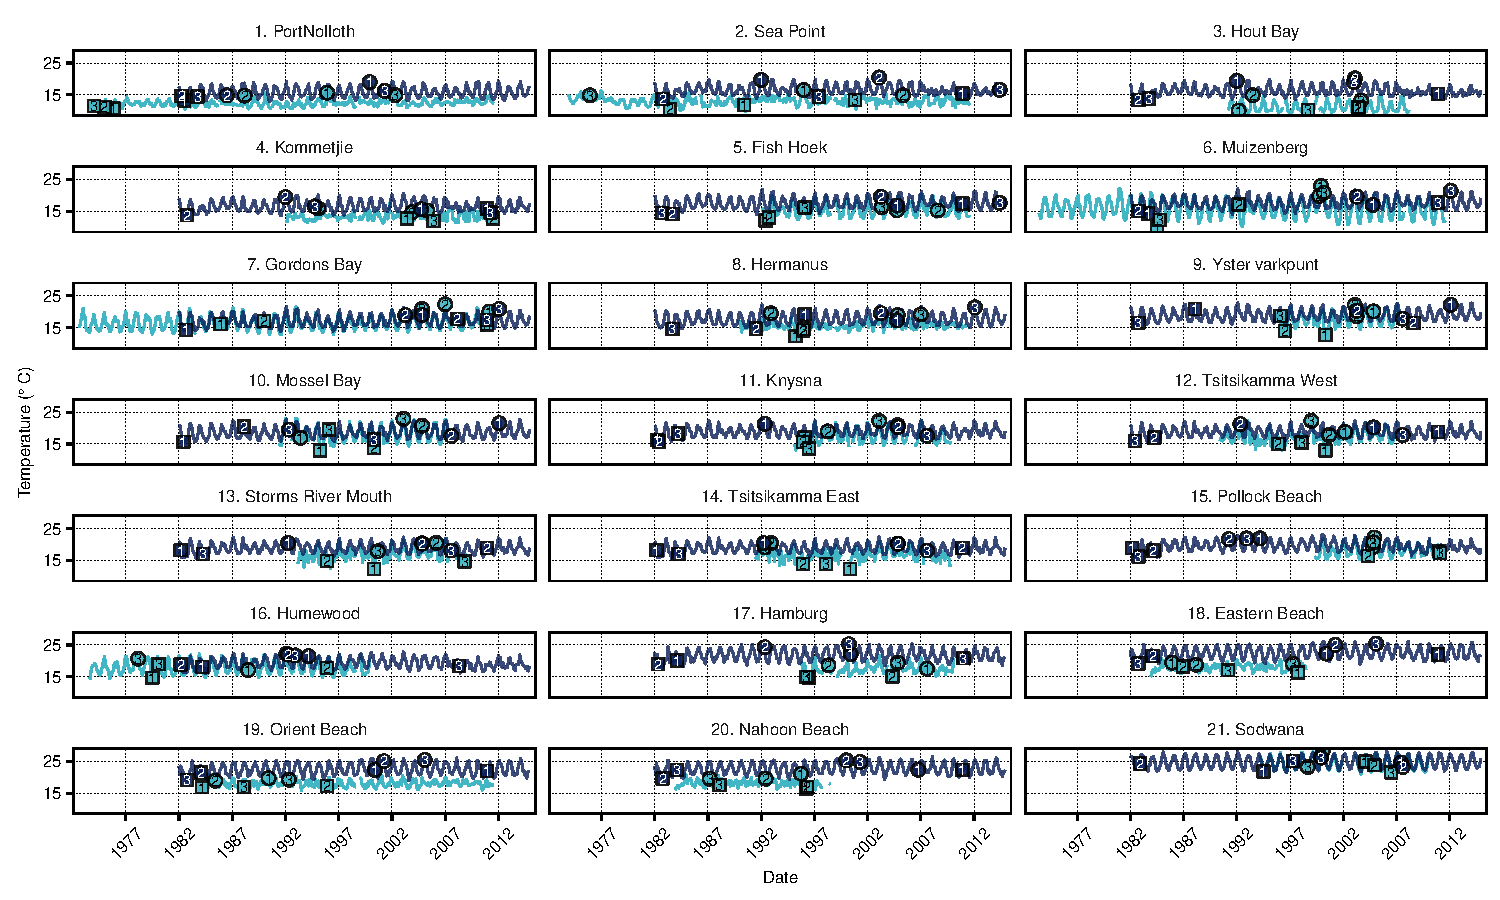
\includegraphics[width=0.50\textwidth]{figure2.pdf}
\caption{The daily temperature values for each \emph{in situ} time series (grey) used in this study and the corresponding OISST time series (black) extracted for comparison as seen in \Cref{fig:Figure1}. The top three MHWs are indicated by circles (with the rank inside) for each site as judged by greatest cumulative intensity. The top three MCSs for each site are indicated by squares (with the rank inside). Sites 1 -- 4 represent the west coast, sites 5 -- 17 represent the south coast and sites 18 -- 21 represent the south coast.} \label{fig:Figure2}
\end{figure}

As with the MHWs, the largest three MCSs from the \emph{in situ} data were also found on the south coast (\Cref{table5}). Maintaining the pattern seen with the MHWs, the largest heat waves on the west coast were the next largest three events for the entire coastline with the three largest events from the east coast being smaller than the other two coastal sections (\Cref{table5}). The mean cumulative intensity for MCSs over the entire coastline was 26.45(\degree C x days) with a standard deviation of 24.25(\degree C x days).

\begin{table}[]
\caption{\small The three largest MCSs per coast from the \emph{in situ} data. Column descriptions may be found in the caption for \Cref{table4}.}
\label{table5}
\centering
\tiny
\begin{tabular}{llcccc}
\hline
 coast & site & start date & duration [days] & intMean [\degree C] & intCum [\degree C x days] \\ 
  \hline
  west & Sea Point & 1990-06-23 & 44 & 2.88 & 126.60 \\ 
  west & Sea Point & 1983-06-10 & 39 & 2.84 & 110.90 \\ 
  west & Sea Point & 2000-11-28 & 23 & 3.70 & 85.04 \\ 
  south & Muizenberg & 1984-07-14 & 63 & 2.92 & 183.70 \\ 
  south & Muizenberg & 1992-03-24 & 56 & 2.78 & 155.60 \\ 
  south & Ystervarkpunt & 2000-05-11 & 51 & 2.94 & 150.10 \\ 
  east & Sodwana & 2004-02-12 & 17 & 3.25 & 55.20 \\ 
  east & Orient Beach & 1984-03-31 & 13 & 3.73 & 48.44 \\ 
  east & Orient Beach & 1995-12-6 & 15 & 3.01 & 45.13 \\ 
  \hline
  \end{tabular}
\end{table}

As can be seen in \Cref{fig:Figure2}, the three largest events occurring for each time series within the OISST dataset are largely different from the \emph{in situ} dataset and show a greater amount of co-occurrence for neighbouring coastal stations than the corresponding \emph{in situ} time series. The pattern seen in the \emph{in situ} data of the largest MHWs and MCSs occurring on the south, west and east coasts respectively is also not repeated with the OISST dataset. Whereas the largest MHW occurred on the south coast in the OISST data, the three largest MHWs from the west coast were larger than the second and third largest events from the south coast (\Cref{table6}). The three largest MHWs from the east coast again came in below the other coasts(\Cref{table6}). The coastal average for the MHWs from the OISST data was smaller than its \emph{in situ} counterpart at 18.65(\degree C x days) and a standard deviation of 15.10(\degree C x days).

\begin{table}[]
\caption{\small The three largest MHWs per coast from the OISST data. Column descriptions may be found in the caption for \Cref{table4}.}
\label{table6}
\centering
\tiny
\begin{tabular}{llcccc}
\hline
 coast & site & start date & duration [days] & intMean [\degree C] & intCum [\degree C x days] \\ 
  \hline
  west & Sea Point & 1992-01-21 &  39 & 2.96 & 115.60 \\ 
  west & Hout Bay & 1992-01-20 &  36 & 3.15 & 113.50 \\ 
  west & Kommetjie & 2004-10-29 &  53 & 2.03 & 107.40 \\ 
  south & Knysna & 1992-05-3 &  50 & 2.41 & 120.40 \\ 
  south & Fish Hoek & 2004-10-30 &  53 & 1.92 & 101.60 \\ 
  south & Pollock Beach & 1994-03-27 &  31 & 3.19 & 99.05 \\ 
  east & Nahoon Beach & 2006-10-21 &  25 & 1.81 & 45.34 \\ 
  east & Eastern Beach & 2000-06-24 &  26 & 1.58 & 41.12 \\ 
  east & Orient Beach & 2000-06-24 &  26 & 1.58 & 41.12 \\ 
  \hline
  \end{tabular}
\end{table}

The largest MCSs from the OISST data (\Cref{table7}) are much less clearly ranked than their \emph{in situ} counterparts (\Cref{table5}). The three largest MCSs on the east coast, like with both datasets and both types of events, were smaller than the other two coasts (\Cref{table7}). The first and second largest east coast events both occurred in 2010 making this a particularly warm year. The coastal average and standard deviation for the cummulative intenstiy of the MCSs from the OISST data were much closer to their \emph{in situ} counterparts than the MHWs were at 23.17(\degree C x days) and 23.49(\degree C x days).

\begin{table}[]
\caption{\small The three largest MCSs per coast from the OISST data. Column descriptions may be found in the caption for \Cref{table4}.}
\label{table7}
\centering
\tiny
\begin{tabular}{llcccc}
\hline
 coast & site & start date & duration [days] & intMean [\degree C] & intCum [\degree C x days] \\ 
  \hline
  west & Kommetjie & 2010-12-13 &  54 & -3.92 & -211.90 \\ 
  west & Hout Bay & 2010-12-25 &  41 & -4.06 & -166.30 \\ 
  west & Sea Point & 2010-12-25 &  41 & -3.78 & -154.90 \\ 
  south & Hamburg & 1984-02-5 &  65 & -3.91 & -254.20 \\ 
  south & Storms River Mouth & 1982-03-13 &  60 & -2.79 & -167.30 \\ 
  south & Tsitsikamma East & 1982-03-13 &  60 & -2.79 & -167.30 \\ 
  east & Eastern Beach & 2010-12-26 &  32 & -2.90 & -92.85 \\ 
  east & Orient Beach & 2010-12-26 &  32 & -2.90 & -92.85 \\ 
  east & Eastern Beach & 1984-02-24 &  22 & -3.97 & -87.26 \\ 
  \hline
  \end{tabular}
\end{table}

The temperature values on the dates of the largest MHW and MCS for the west and south coasts from the \emph{in situ} data may be seen concurrently with the temperature values from the same OISST time series in \Cref{fig:Figure3}. One may see that when the largest events were occurring in the \emph{in situ} data, nothing of note was occurring within the OISST data.

\begin{figure}
\centering 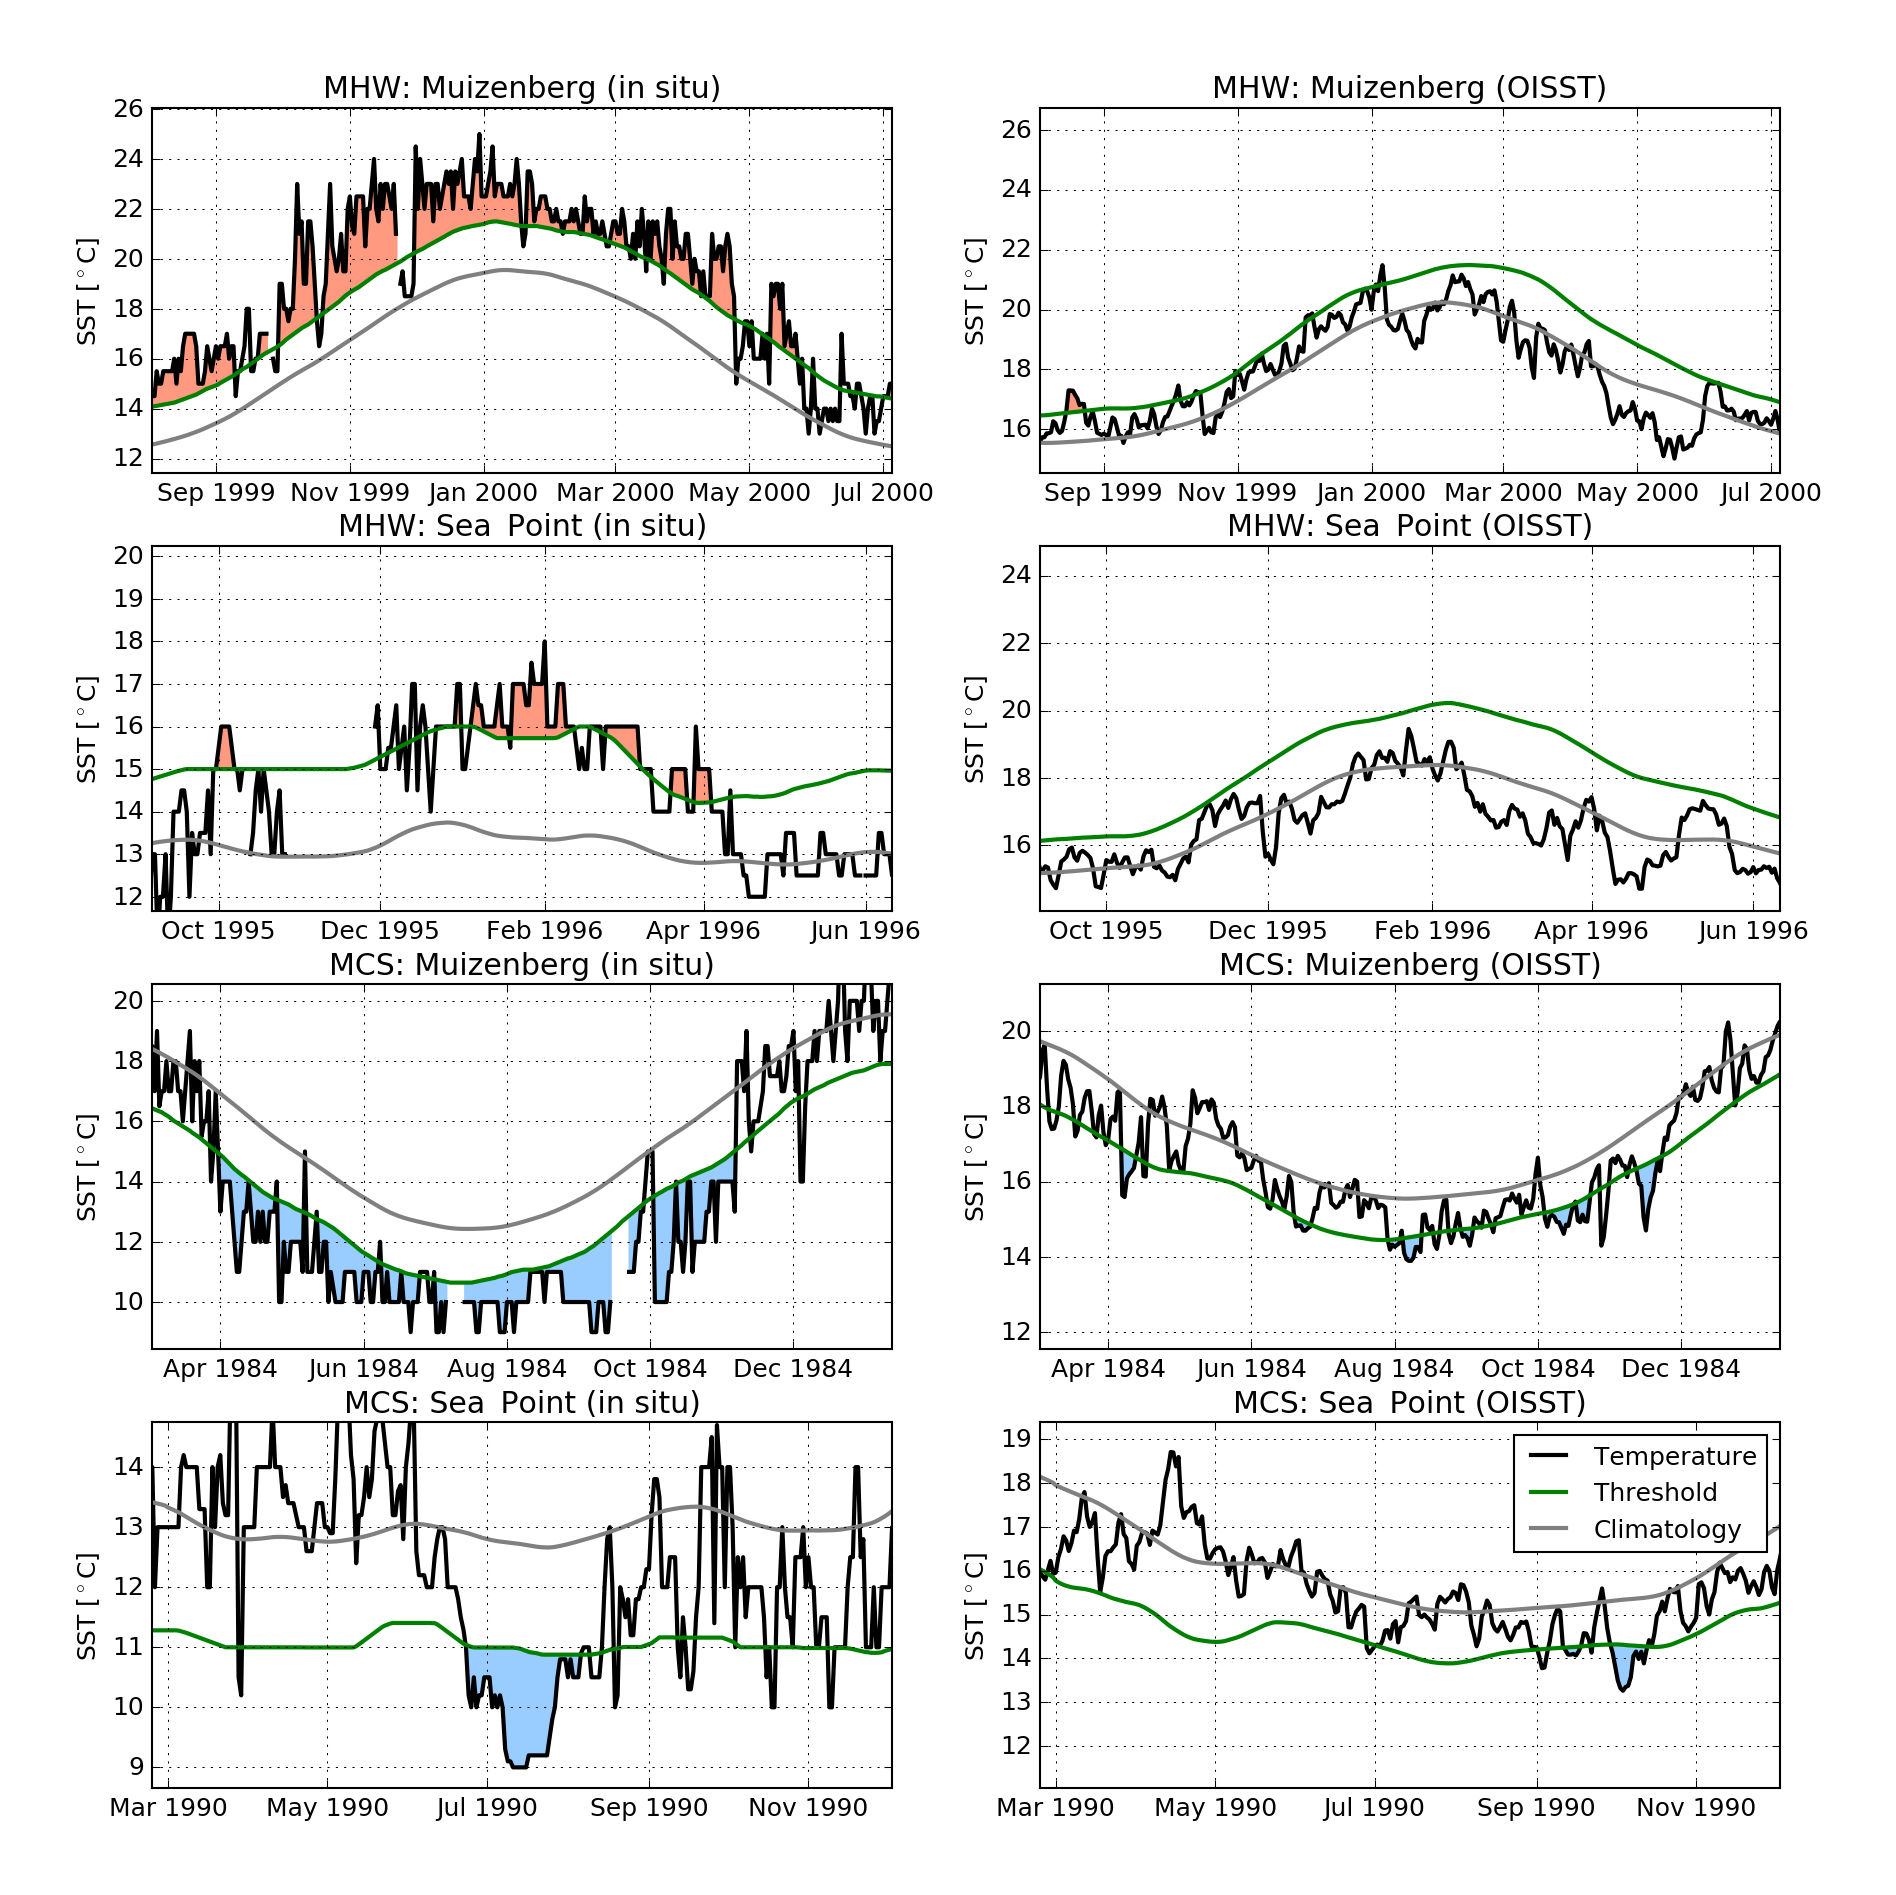
\includegraphics[width=1.0\textwidth]{figure3.png}
\caption{These eight panels show the profiles for the four events depicted in Figure YXZ. The left column shows the \emph{in situ} event while the right column shows the OISST temperature occurring on the same dates. The top row shows the largest MHW that occurred on the south coast while the second row shows the largest MHW that occurred on the west coast. The bottom two rows show the largest MCS that occurred on the south and west coasts respectively.} \label{fig:Figure3}
\end{figure}

\subsection{Co-occurrence rates}\todo{I feel like I need to describe more of these results here. I also need to calculate statistical significance between the different coastlines/lags/directions/events.}
The proportion of co-occurrence for events between the datasets for each coastal section may be seen in \Cref{fig:Figure4}. We see that as the length of lag is increased the proportion of co-occurrence increases linearly for both MHWs and MCSs with the largest increase in co-occurrence on the south coast and the least on the west. The directionality of the lag also affects the co-occurrence of events. A lag window before the \emph{in situ} event gave higher rates of co-occurrence for all three coastal sections for both MHWs and MCSs when all events were compared. This pattern changed when the smaller events were screened from comparison. When only the largest half of the events were checked for co-occurrence a lag window after the \emph{in situ} event gave larger rates of co-occurrence. The overall proportion of co-occurrence for MHWs is greater than that of MCSs. There is no co-occurrence for the largest MCSs between the datasets, whereas several of the time series on the south coast show co-occurrence for their most extreme MHWs. Interestingly the rates of co-occurrence for these largest MHWs was greater when the \emph{in situ} event preceded the OISST event.

\begin{figure}
\centering 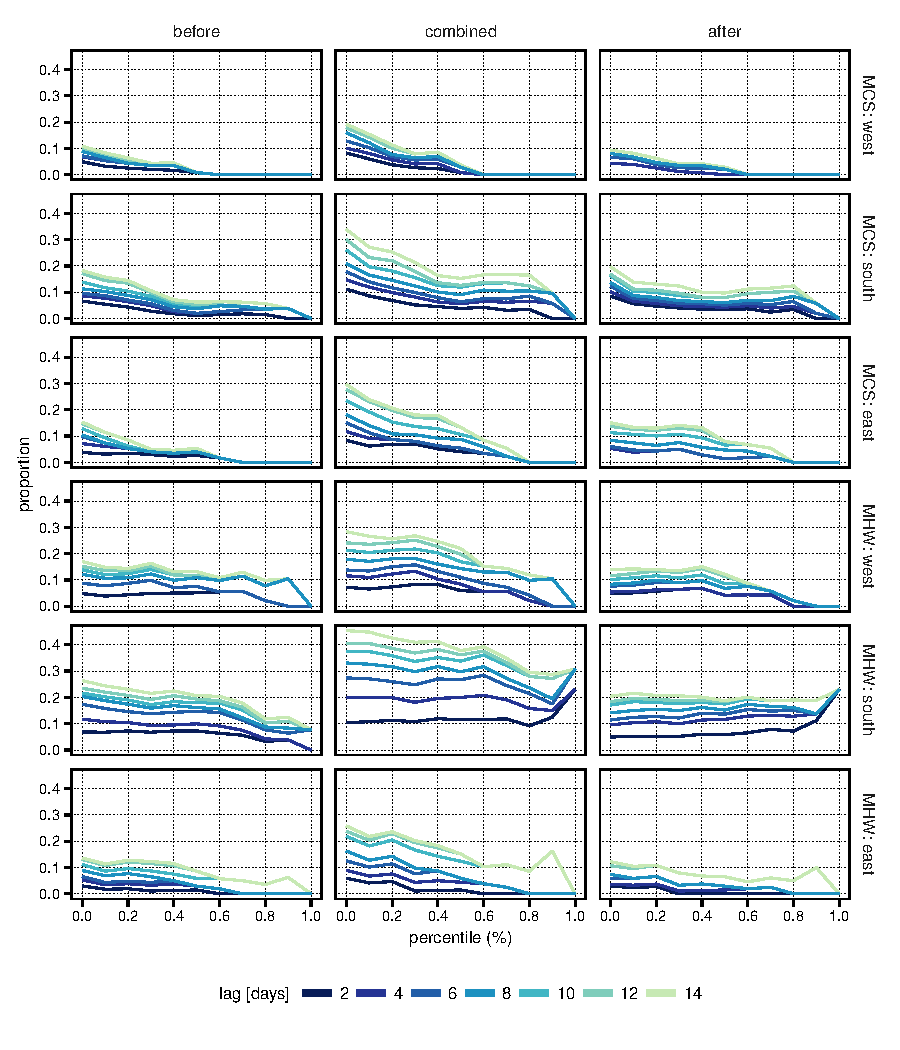
\includegraphics[width=1.0\textwidth]{figure4.pdf}
\caption{Proportion of MHW and MCS co-occurrence between \emph{in situ} and OISST datasets for each coastal section. The left column denotes the proportion of co-occurrence when only events in the OISST data occurring on dates preceding the \emph{in situ} event are used. The left column shows the proportion of co-occurrence when only OISST events occurring after the \emph{in situ} date are compared. The central column shows the overall proportion of co-occurrence when the lag window is extended in both directions. The $x$-axis indicates the size of the events, based on percentiles, used for calculating the co-occurrence proportions. As the smaller events are removed from the pool of comparison, the proportion of co-occurrence diminishes.} \label{fig:Figure4}
\end{figure}

\section{Discussion}

\subsection{Events}
Having never been calculated before, it was not yet known that every time series from each coastal section of South Africa experiences on average more than one MHW and one MCS per year. It was surprising to find that the mean intensity of MCSs on the south coast was significantly larger (\emph{p} = XX) than the west coast, which is in an EBUS. Even though the south coast is known to be the most volatile of the three coasts, it was not expected that the duration (days) of both the MHWs and MCSs occurring there would be significantly longer (\emph{p} = XX) than the other two coasts. From these results we may now hypothesise that there is an additional driver on the south coast affecting the extreme events there that is not present on the other two coastal sections. It was assumed that the east coast would experience the fewest and least intense events. Whereas the duration of its events were significantly smaller than the other two coasts (\emph{p} = XX), the frequency and mean intensity of its MHWs and MCSs was not the smallest found. This means that every portion of the coastline has the potential to experience an event strong enough to affect its species assemblage and/or local ecology.

The difference between the \emph{in situ} and OISST datasets was also striking. One may see in Table 2 and Table 3 that the patterns presented by the data are intrinsically different, it is not simply a matter of the statistical significance between the statistics. The OISST data show many weak events occurring often whereas the \emph{in situ} dataset shows fewer, stronger events. This implies that events occurring in the different datasets are unrelated, and any co-occurrence is simply by chance. Besides this difference, both datasets tend to show that the south coast has the longer and more intense results than the other two coastal sections, but this too is not a consistent result. Before calculating the proportions of co-occurrence, it was already clear from these results that the events occurring within the OISST data would differ from the \emph{in situ} data.

Another important difference found between the datasets was that MHWs are shown to be longer and more intense in the \emph{in situ} dataset, whereas the OISST dataset shows MCSs being longer and more intense. This also supports the argument that the events detected by these two datasets are not the same, even when they are found to occur within similar time frames. It is also counter-intuitive to what we expected to find. One would assume that as the \emph{in situ} data are measured at \emph{ca}. 5 m deep on average, which is below the bulk surface layer (\emph{ca}. 0.5 m) that the OISST data measure \cite{Reynolds2002}, they would be predisposed to picking up cold upwelling events and less exposed to thermal heating, which would appear as larger MCSs and smaller MHWs compared to the OISST data. The cause of this discrepancy warrants further research.

This apparent discrepancy also places doubt on the use of MCSs as a proxy for upwelling. If the \emph{in situ} data had recorded longer and/or more intense MCSs than the OISST data it would have shown that the MCS algorithm was detecting more extreme cold events near the coastline, where upwelling is known to occur \cite{Hutchings2009, Lutjeharms2000}. Instead the results show that offshore MCS are, on average, longer and more intense. It is the suggestion of the authors that using the MCS algorithm to detect upwelling be done with extreme caution. The MCS algorithm detects cold events based on their intensity outside of a locally produced climatology, and because most upwelling occurs at seasonally predictable times, the cold events detected here are likely due to other factors.

\subsection{Top three events}
It was hypothesised that the south coast would experience the most extreme events as measured by cumulative intensity, but it was unanticipated that these events would be so much larger than the other two coastal sections. On the opposite side of the coin, it was hypothesised that the east coast would experience the least extreme events however, besides the largest two MHWs recorded, very few of the events are greater than the coastal average.

The disagreement between the \emph{in situ} and OISST datasets continued into the detection of the top three events along the coastline. The pattern of event sizes within the \emph{in situ} data are very clear in that the south coast is much more volatile than the west and east coasts in that order. The OISST data are less conclusive on whether the south or west coast experiences the most extreme events, but it is apparent from all of the analyses from both datasets that the east coast experiences very few extreme MHWs or MCSs. Indeed, these findings support the hypothesis that the east coast is the most stable of the three coasts in that in both datasets the most extreme events occurring here barely exceed the coastal mean for cumulative intensity.

The sites along the south coast could be further divided into those within False Bay (Sites 5--7) and those on the Agulhas Bank (Sites 8--17). False Bay, which is ~50 km across, is situated within the transition zone between the Benguela and Agulhas Currents \cite{Smit2013}. Many satellite temperatures products therefore inadequately resolve the SST within this body of water (cite.). This is problematic as it is important to precisely monitor the large ranges in temperature this area experiences (cite.) as it is important both ecologically (cite.) and to the many stakeholders that use this embayment. Two of the three largest MHWs and MCSs from the \emph{in situ} dataset were recorded within False Bay, whereas only one large MHW and no MCSs were detected with the OISST dataset. This illustrates the problem of using satellite temperature data for coastal ecology.

The example of the discrepancies for the size of the events recorded in False Bay also serves to illustrate the usefulness of satellite SST data to detect events near the coastline. For example, Roberts (2004) \cite{Roberts2005} argues for a wind forced coastal upwelling cell near Tsitsikamma (Sites 12–-14). That these three sites show greater cumulative intensities for MCSs than all but one time series for the OISST dataset supports the hypothesis of such a coastal upwelling cell. This is an intriguing use of the MCS algorithm to validate multiple competing hypotheses that as of yet may not have been able to be tested in any other way. \todo{Need to relate MCSs not showing upwelling though...}

\subsection{Co-occurrence rates}
As one may see in \Cref{fig:Figure4}, when looking at the the lag window before the \emph{in situ} events occurred, the rates of co-occurrence for MCSs are much lower than for the MHWs. This shows that more MHWs are likely being caused by meso-scale activity than MCSs, as was expected. This finding is supported further by comparing the rates of co-occurrence for MCS lagged before and after the \emph{in situ} event occurred. More MCS from the OISST data are shown to occur after the \emph{in situ} events for all coastal sections. The co-occurrence rates of MHWs before and after the \emph{in situ} events are similar.

One may also infer from the result that the proportions of co-occurrence for time series on the south coast being much larger than the other two coasts is caused by the much higher level of influence from meso-scale phenomena occurring on the Agulhas Bank. We also see that there is a higher proportion of co-occurrence for the larger MHWs and MCSs on the south coast when a lag window after the \emph{in situ} event is used (\Cref{fig:Figure4}). This supports the argument that events originating in the nearshore are then propagating out onto the Agulhas Bank and affecting the oceanography there more often than meso-scale events originating on the Agulhas Bank are affecting the nearshore environment. The overall low rates of co-occurrence for all three coastal sections reinforces the argument that it is not the meso-scale phenomena of the open ocean around the coastline that is causing extreme events in the nearshore.

The very low proportion of co-occurrence between the datasets, and the decline in the proportion as the smaller events are screened out is strong evidence against the hypothesis that meso-scale activity, both warm and cold, is causing nearshore extreme thermal events. The small increases in co-occurrence as outlined above do imply that there is some relationship between the inshore and offshore, but that some other variable(s) is having a greater effect on the inshore. This is likely atmospheric forcing (cite.).

\subsection{Climate change}
As MHWs and MCSs are temperature related phenomena we would be remiss not to discuss the potential of our findings in relation to climate change. The count of the MHWs and MCSs occurring throughout the coastline is less telling in this regard than the trend in these events themselves. Although the \emph{in situ} time series used in this investigation are too short to draw adequate conclusions on the trends seen in MHWs and MCSs, \todo{But we can do this using the OISST data --- and we should!} one can see in \Cref{fig:Figure2} that most sites have their top three MCSs in the first half of the time series whereas the top three MHWs occur in the second half of the time series. As the algorithm used to calculate these events is based on percentiles, it stands to reason that as the mean temperature of South Africa's coastal waters increases by 0.1\degree C per decade on average (Schlegel and Smit, in press)\todo{Not sure how to reference this...}, that there will be an increase in MHWs and a decrease in MCSs. The gradual mean increase in temperature will cause the algorithm used here to be biased in its detection of MHWs as time progresses simply because temperatures are generally warmer in the later half of the time series therefor, the chances of the algorithm detecting a MHW increases because the base temperature from which the MHW will be fluctuating from will be greater than the beginning of the time series. Ultimately, for the species and ecosystems experiencing this increase in duress, the semantic argument of the viability of percentiles provides little solace. \todo{Nice concluding statement here!}

\subsection{Conclusion}
Given that the MHW algorithm is based on the percentiles found within each time series and not on arbitrarily decided minimum or maximum thresholds, one will always find a certain number of MHWs and MCSs. This is evident in the results of our analysis (\Cref{table2} and \Cref{table3}) in that every time series used from both datasets experiences on average at least one MHW and MCS per year. Within each dataset, but not between, the lengths of these events are similar throughout the coastline, regardless of the local oceanographic and geographic properties. \todo{This statement needs to be supported by the statistical results of an ANOVA.} It is the cumulative intensity of the events occurring on the different coastal sections that most clearly defines them. We expected to see the most intense MCSs on the west coast as this is part of an EBUS however, the south coast, a region dominated by the warmer Agulhas Current, but with some influence from the colder Benguela, had both the most intense and longest MHWs and MCS in the \emph{in situ} data. Even though it had been hypothesized that the south coast would have intense events, the magnitude of intensity of the events that occurred here over the other coastlines is surprising. \todo{Also perform ANOVA on the cumulative events to support this statement statistically.}

We have also shown that MCSs are not a good indicator for upwelling. As upwelling tends to occur at seasonally predictable times, the MCS algorithm does not consider these events as anomalous. Therefore the MCSs measured here are indicators of non-seasonal or atypical forcing, which is assumed to be largely atmospheric.

As the rates of co-occurrence between \emph{in situ} and OISST data are generally low, this implies that some other force is contributing to extreme inshore events. This is likely due to atmospheric forcing and warrants further research to better understand what is driving the occurrence and intensity of these events.

\section*{References}

\bibliography{MHW}

\end{document}